\documentclass{article}

\usepackage[english]{babel}


\usepackage[a4paper,top=2cm,bottom=2cm,left=3cm,right=3cm,marginparwidth=1.75cm]{geometry}
\usepackage{amsmath}
\usepackage{graphicx}
\usepackage[colorlinks=true, allcolors=blue]{hyperref}
\usepackage[normalem]{ulem}
\usepackage{tabularx}
\usepackage{booktabs}
\usepackage{listings}
\usepackage{lipsum}  

\lstdefinestyle{sqlStyle}{
  language=SQL,
  basicstyle=\ttfamily\small,
  keywordstyle=\color{blue},
  commentstyle=\color{gray},
  stringstyle=\color{orange},
  numbers=left,
  numberstyle=\tiny\color{gray},
  stepnumber=1,
  tabsize=4,
  showspaces=false,
  showstringspaces=false
}


\title{Documentazione Tecnica Progetto Basi Di Dati 2022-2023}
\author{Martino Francesco Leone}
\date{Agosto 2023}

\begin{document}
\maketitle

\tableofcontents

\section{Introduzione}
Di seguito, la presente documentazione tecnica procederà a illustrare, come richiesto, tutte le scelte implementative che hanno portato allo sviluppo della base di dati, insieme alle scelte di progettazione concettuale e logica della stessa, nonché gli aspetti metodologici adottati.

Verranno inoltre illustrati tutti i trigger e le funzioni implementati, e sarà fornita una definizione di come ciascun componente sia stato interpretato in relazione alla traccia d'esame\footnote{Per "traccia d'esame" si fa riferimento al compito assegnato dal professore e pubblicato su Ariel, aggiornato al 25 agosto 2023; si presume che tale traccia sia nota al lettore}.

Si procederà ora con la dettagliata esposizione delle suddette informazioni.

\include{definizioneentità}
\section{Diagramma Concettuale}\label{concettuale}
\begin{figure}[ht]
    \centering
    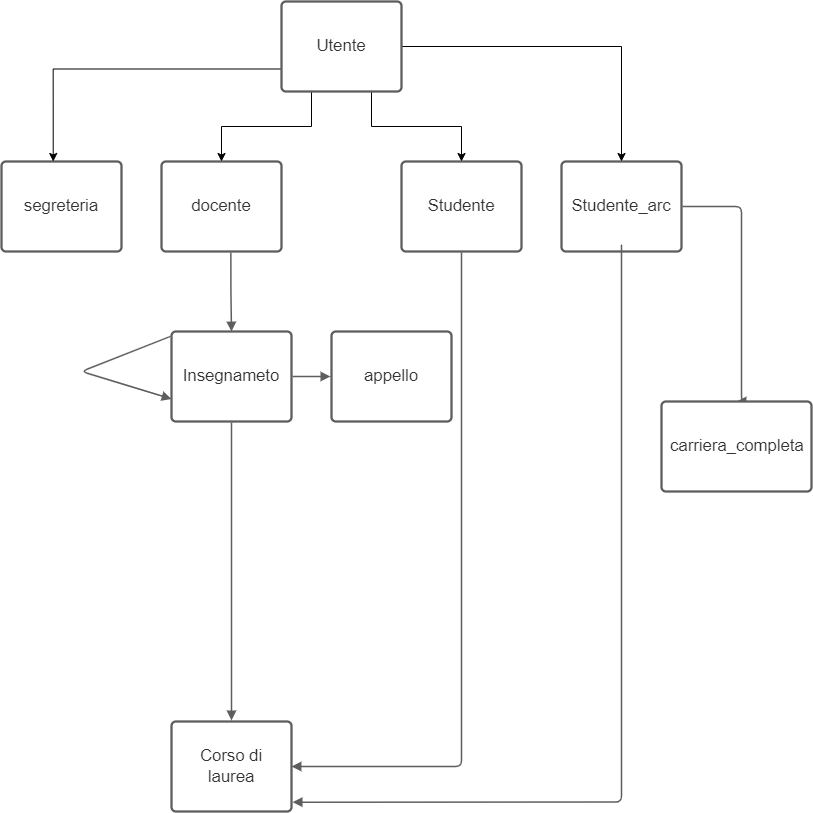
\includegraphics[width=0.5\linewidth]{images/concettuale-1.png}
    \caption{Prima versione del diagramma concettuale}
    \label{fig:concettuale1}
\end{figure}
Iniziamo a sviluppare il diagramma concettuale partendo da ciò che possiamo dedurre a una prima lettura della consegna, sapremo che avremo le  seguenti entità:
\begin{itemize}
    \item Utente:
    \begin{itemize}
        \item Segreteria
        \item Docente
        \item Studente
        \item Studente Archiviato
    \end{itemize}
    \item corso di laurea 
    \item Insegnamento
\end{itemize}

\subsection{Utenti}
Per prima cosa concentriamoci su utenti i quale si trovano in una gerarchia e necessità una ristrutturazione:

procederemo con una ristrutturazione verso il basso dove quindi ci assicureremo che ogni entità figlia sia indipentente
\subsection{Insegnamenti}
non necessità di particolari ristrutturazioni se non una specificazione che la relazione con se stessa definisce la propedeuticità  e si tratta di un n-n
\subsection{Corso di Laurea}
non necessità ristrutturazioni
\subsection{Studente}
non necessità ristrutturazioni
\subsection{Appello}
Appello necessita di una grande ristrutturazione in quando necessità un associazione a studente e l'aggiunta di una tabella che permettà l'iscrzione agli studenti che chiameremo sostiene (\ref{sostiene})
\subsection{Archivio}
Per quanto riguarda la gestione della tabella carriera completa segue una ristruttuazione in linea con la struttura esposta nella sezione \ref{archivio}

\subsection{Aggiornamento Diagramma}
applicando quindi le ristrutturazioni sopra citate possiamo illustrare il nuovo diagramma concettuale in figura \ref{fig:concettuale2}
\begin{figure}[ht]
    \centering
    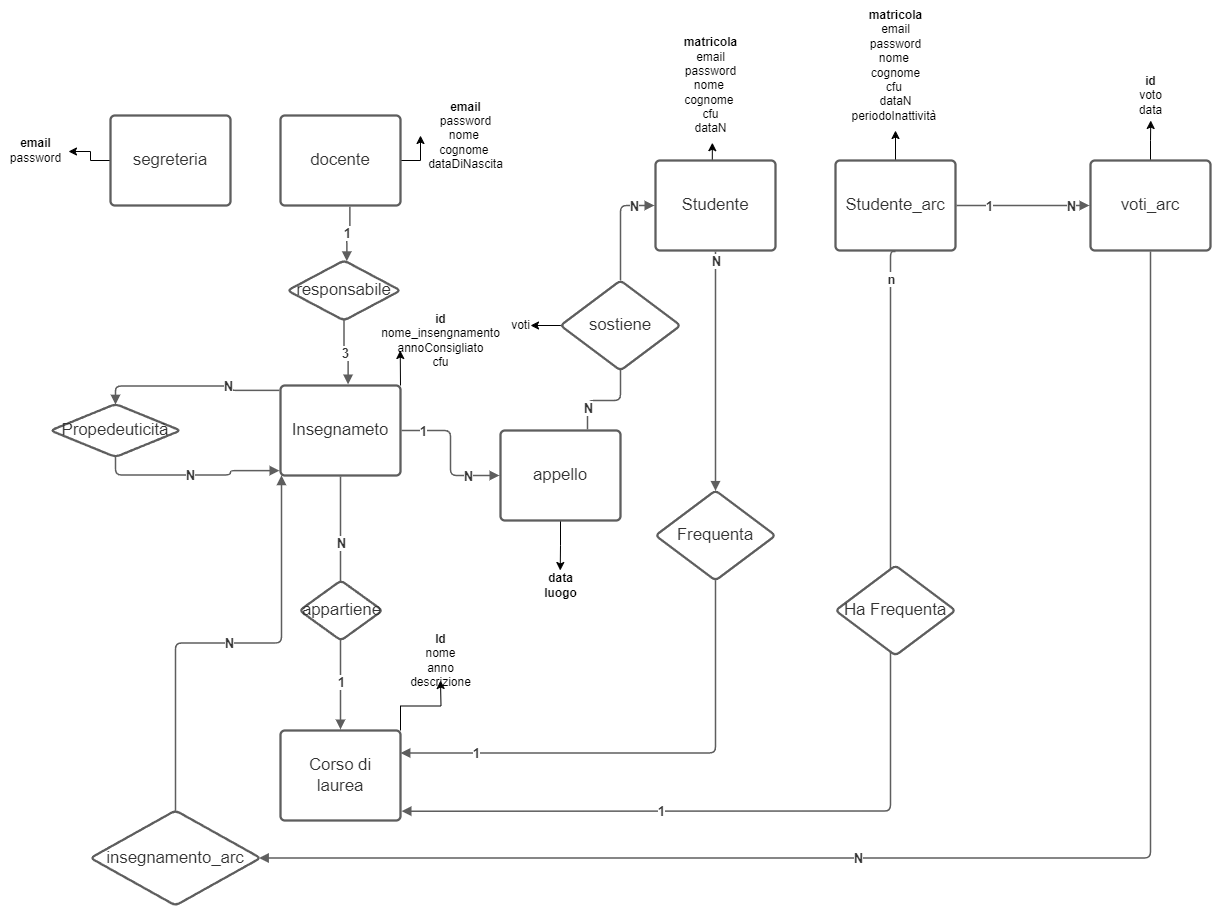
\includegraphics[width=0.8\linewidth]{images/concettuale-2.png}
    \caption{diagramma concettuale definitivo}
    \label{fig:concettuale2}
\end{figure}

Come si può notare sono state aggiunte le propedeuticità per l'insegnamento, è stata creata la relazione sostiene tra studente e appello e l'archivio è stato strutturato
\section{Diagramma Relazionale}
Procediamo ora con lo sviluppo del diagramma relazionale partendo dal concettuale, analiziamo nel dettagli tutte le scelte  implementative\footnote{ci concentreremo princpalmente sulle modifiche più radicali, molte entità infatti non verranno alterare} fatte in figura \ref{fig:diagrammaRelazionale}
\begin{figure}
    \centering
    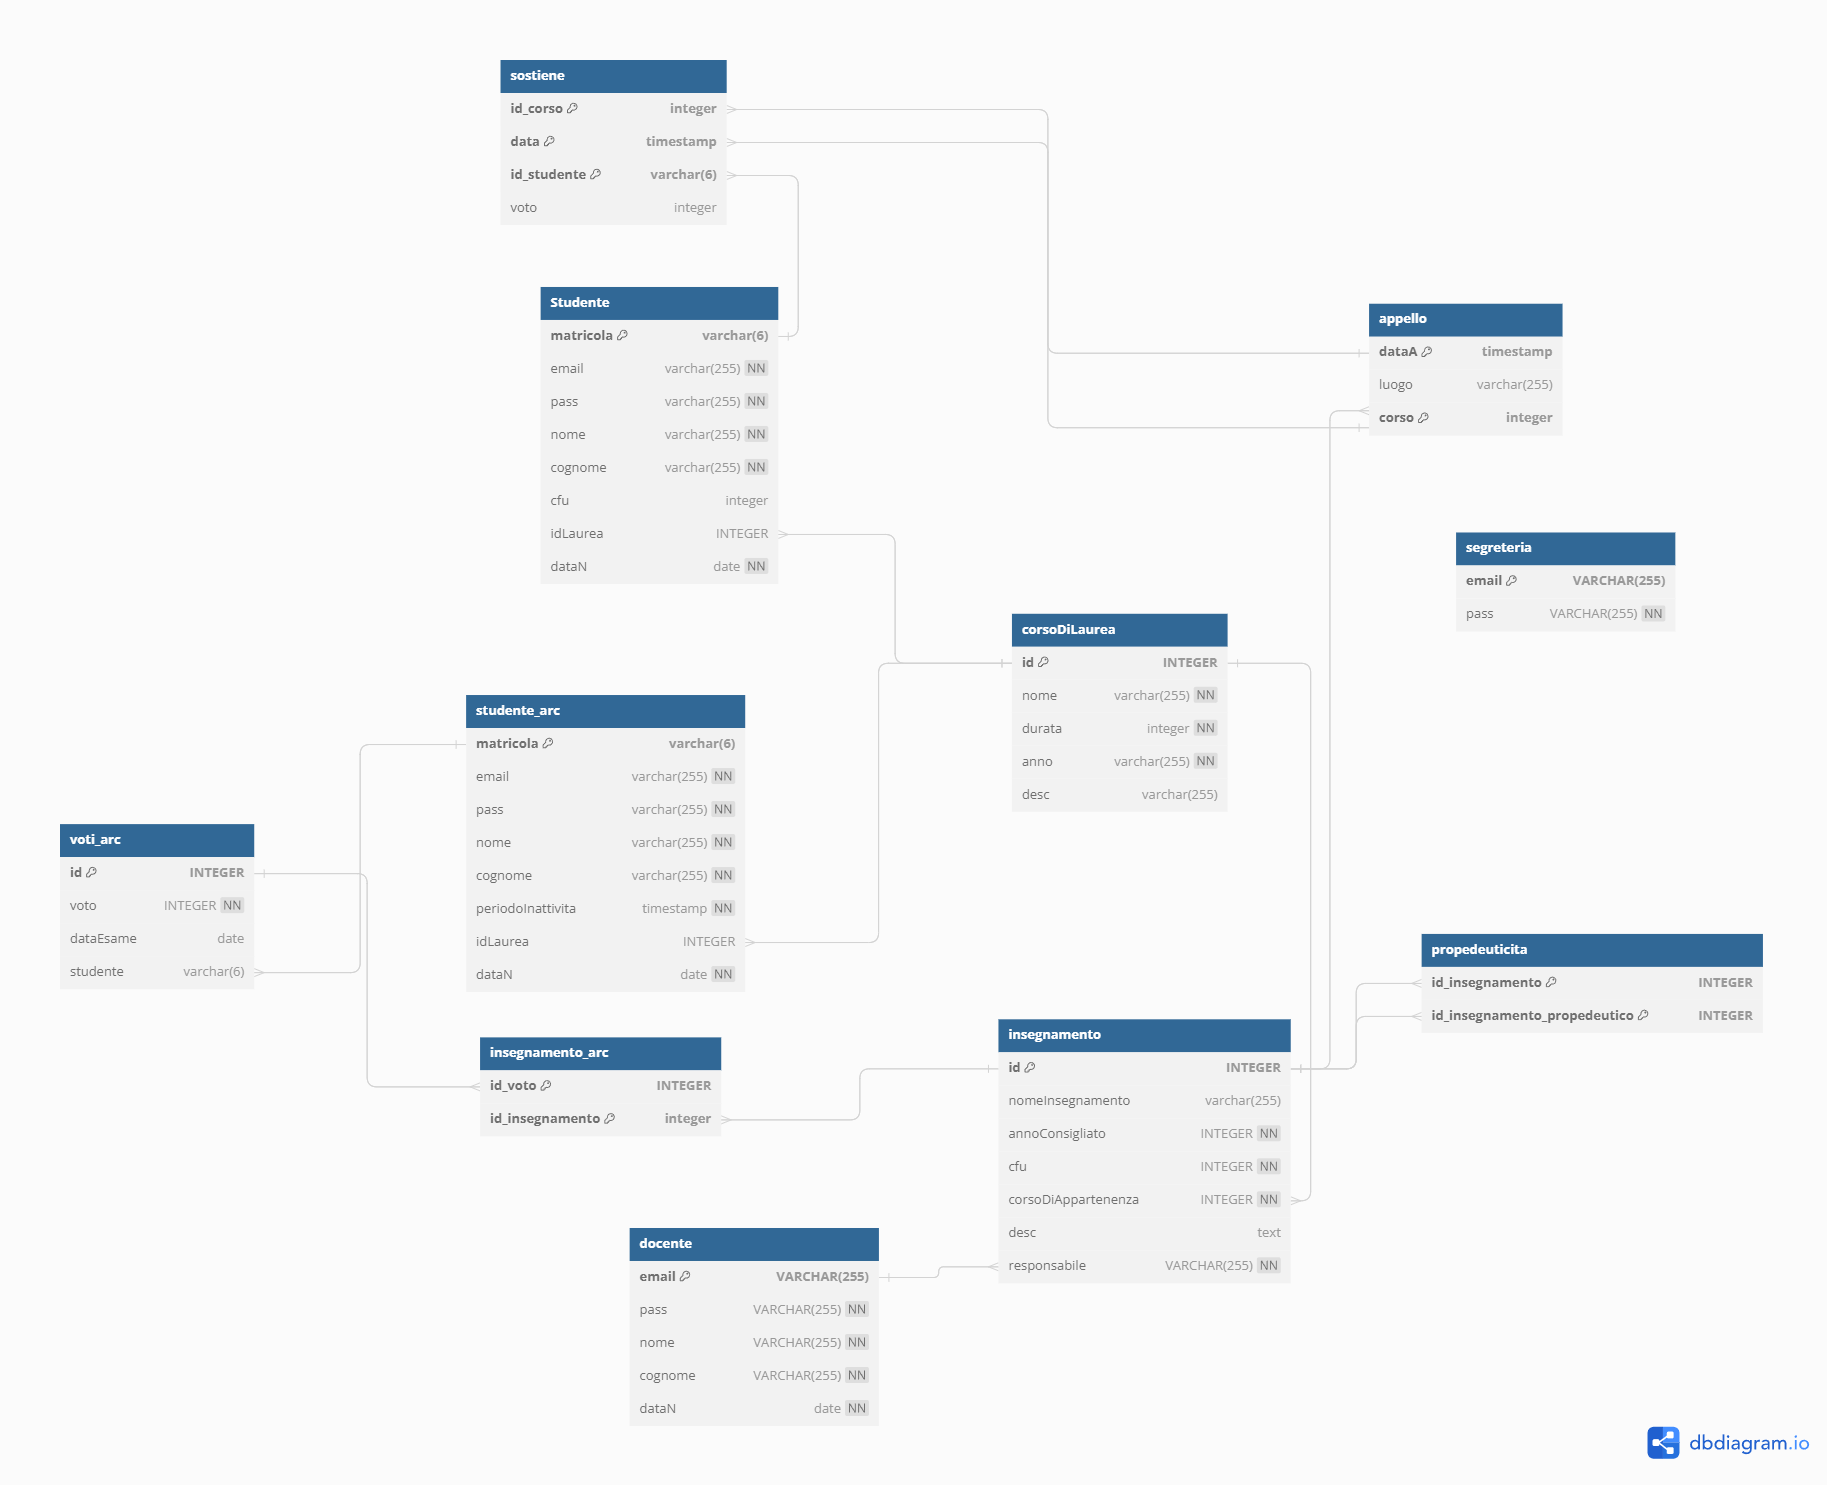
\includegraphics[width=0.9\linewidth]{images/relazionale.png}
    \caption{Diagramma Relazionale}
    \label{fig:diagrammaRelazionale}
\end{figure}
\subsection{Entità invariate}
Mostriamo ora le entità che non hanno ricevuto modifice significative: 
\begin{itemize}
    \item \textbf{corsoDiLaurea}: \underline{id} un integer auto increment che identifica il corso di laurea 
    \item \textbf{Studente}: la sua struttura rimane la stessa della sezione \ref{Studente} con la differenza che:
    \begin{itemize}
        \item \underline{matricola}: chiave primaria che identifica unviocamente lo studente  
        \item \dashuline{idLaurea}: chiave esterna riferita ad un corso di laurea che permette di identificare il corso di laurea a cui è iscritto 
    \end{itemize}
    \item \textbf{docente}: \underline{email} definisce unicovemente il docente con la struttura \textit{nome.cognomeN@segreteria.com}\footnote{dove \textit{N} definisce un numero intero generato tra 1,100}
    \item \textbf{Insegnamento}: 
    \begin{itemize}
        \item \textbf{id}  un integer auto increment che identifica l'insegnamento
        \item  \dashuline{responsabile}: chiave esterna che si riferisce all'insengnamente responsabile del corso, per motivi che illustreremo nello sezione \ref{createDocente} sarà fondamentale assegnare a responsabile un \textit{CONTRAINT DEFERRABLE INITIALLY DEFERRED}

    \end{itemize}
    \item \textbf{appello}:
    \begin{itemize}
        \item \underline{dataA}
        \footnote{dataA è chiave primaria in modo da rispettare il vincolo del singolo esame in un giorno per corso}
        : chiave primaria che rappresenta la data in cui viene sostenuto l'esame
        \item \dashuline{\underline{corso}} chiave primaria di appello e chiave esterna di insegnamento
    \end{itemize}
    \item \textbf{segreteria}: \underline{email} chiave primaria (vedi \ref{segreteria} per spiegazione)
\end{itemize}
\subsection{Moficiche}
Vediamo ora le entità che hanno subito cambiamenti radicali
\subsubsection{Gestione Archivio}
L'archivio è gestito da una serie da alcune entità che ora vedremo e analizzeremo nel dettaglio:
\begin{itemize}
    \item \textbf{studente\_arc}: \underline{email} stesso formato dello studente
    \item \textbf{voti\_arc}: \underline{id} definisce univicoamente il voto (vedi \ref{voto archivio})
    \item \textbf{insegnamento\_arc}:
    \begin{itemize}
        \item \dashuline{\underline{id\_voto}}: chiave primaria e chiave esterna su \textit{voti\_arc}
        \item \dashuline{\underline{id\_insengamento}}: chiave primaria e chiave esterna su \textit{insegnamento}
    \end{itemize}
    lo scopo di quest'entità emettere in relazione voti\_arc e insegnamento  in quanto essi hanno un rapporto n-n
\end{itemize}
\subsubsection{sostiene}
Quest'entità è forse quella che di più viene alterata, la sua struttua infatti diventa:
\begin{itemize}
    \item \dashuline{\textbf{id\_corso}}: chiave primaria e chiave esterna rispetto ad appello 
    \item \dashuline{\textbf{data}}:chiave primaria e chiave esterna rispetto ad appello 
    \item \dashuline{\textbf{id\_studente}}: chiave primaria e chiave esterna rispetto allo studente iscritto
\end{itemize}
\section{Struttua Data Base}

Definiamo quindi ora tutte le tabelle con i rispettivi campi nel dettaglio 
\begin{table}[ht]
\centering
\caption{Tabella Docente}
\begin{tabularx}{\textwidth}{lX}
\toprule
\textbf{Campo} & \textbf{Descrizione} \\
\midrule
email & VARCHAR(255) - Chiave primaria \\
pass & VARCHAR(255) - Non nullo \\
nome & VARCHAR(255) - Non nullo \\
cognome & VARCHAR(255) - Non nullo \\
dataDiNascita & DATE \\
\bottomrule
\end{tabularx}
\label{tab:docente}
\end{table}

\begin{table}[ht]
\centering
\caption{Tabella Segreteria}
\begin{tabularx}{\textwidth}{lX}
\toprule
\textbf{Campo} & \textbf{Descrizione} \\
\midrule
email & VARCHAR(255) - Chiave primaria \\
pass & VARCHAR(255) - Non nullo \\
root & boolean - Non nullo \\

\bottomrule
\label{tab:segreteria}

\end{tabularx}
\end{table}


\begin{table}[ht]
\centering
\caption{Tabella CorsoDiLaurea}
\begin{tabularx}{\textwidth}{lX}
\toprule
\textbf{Campo} & \textbf{Descrizione} \\
\midrule
id & SERIAL - Chiave primaria \\
nome & VARCHAR(255) - Non nullo \\
durata & INTEGER - Non nullo \\
anno & VARCHAR(255) - Non nullo \\
desc & text - Non nullo \\

\bottomrule
\label{tab:corsoDiLaurea}

\end{tabularx}
\end{table}


\begin{table}[ht]
\centering
\caption{Tabella Insegnamento}
\begin{tabularx}{\textwidth}{lX}
\toprule
\textbf{Campo} & \textbf{Descrizione} \\
\midrule
id & SERIAL - Chiave primaria \\
nomeInsegnamento & VARCHAR(255) \\
annoConsigliato & INTEGER - Non nullo \\
cfu & INTEGER \\
desc & TEXT\\
corsoDiAppartenenza & INTEGER - Chiave esterna, riferisce a "corsoDiLaurea" ("id") - Non nullo \\

responsabile & VARCHAR(255) - Chiave esterna, riferisce a "docente" ("email") \\

\bottomrule
\label{tab:insegnamento}

\end{tabularx}
\end{table}

\begin{table}[ht]
\centering
\caption{Tabella Propedeuticità}
\begin{tabularx}{\textwidth}{lX}
\toprule
\textbf{Campo} & \textbf{Descrizione} \\
\midrule
id\_insegnamento & INTEGER - Chiave esterna, riferisce a "insegnamento" ("id") \\
id\_insegnamento\_propedeutico & INTEGER - Chiave esterna, riferisce a "insegnamento" ("id") \\
\bottomrule
\label{tab:propedeuticità}

\end{tabularx}
\end{table}


\begin{table}[ht]
\centering
\caption{Tabella Studente}
\begin{tabularx}{\textwidth}{lX}
\toprule
\textbf{Campo} & \textbf{Descrizione} \\
\midrule
matricola & VARCHAR(6) - Chiave primaria \\
email & VARCHAR(255) - Unico, non nullo \\
pass & VARCHAR(255) - Non nullo \\
nome & VARCHAR(255) - Non nullo \\
cognome & VARCHAR(255) - Non nullo \\
cfu & INTEGER - Default 0 \\
idLaurea & INTEGER - Chiave esterna, riferisce a "corsoDiLaurea" ("id") \\
dataN & DATE - Non nullo \\
\bottomrule
\label{tab:studente}

\end{tabularx}
\end{table}



\begin{table}[ht]
\centering
\caption{Tabella Appello}
\begin{tabularx}{\textwidth}{lX}
\toprule
\textbf{Campo} & \textbf{Descrizione} \\
\midrule
dataA & TIMESTAMP \\
luogo & VARCHAR(255) \\
corso & INTEGER - Chiave esterna, riferisce a "insegnamento" ("id") \\
\bottomrule
\label{tab:appello}

\end{tabularx}
\end{table}

\begin{table}[ht]
\centering
\caption{Tabella Sostiene}
\begin{tabularx}{\textwidth}{lX}
\toprule
\textbf{Campo} & \textbf{Descrizione} \\
\midrule
id_corso & INTEGER \\
data & TIMESTAMP \\
id_studente & VARCHAR(6) - Chiave esterna, riferisce a "Studente" ("matricola") \\
voto & voto \\
\bottomrule
\label{tab:sostiene}
\end{tabularx}
\end{table}


\begin{table}[ht]
\centering
\caption{Tabella Studente\_arc}
\begin{tabularx}{\textwidth}{lX}
\toprule
\textbf{Campo} & \textbf{Descrizione} \\
\midrule
matricola & VARCHAR(6) - Chiave primaria \\
email & VARCHAR(255) - Unico e non nullo \\
pass & VARCHAR(255) - Non nullo \\
nome & VARCHAR(255) - Non nullo \\
cognome & VARCHAR(255) - Non nullo \\
cfu & INTEGER - Predefinito a 0 \\
periodoInattivita & INTERVAL \\
idLaurea & INTEGER - Chiave esterna, riferisce a "corsoDiLaurea" ("id") \\
dataN & DATE - Non nullo \\
\bottomrule
\label{tab:studenteArc}
\end{tabularx}
\end{table}

\begin{table}[ht]
\centering
\caption{Tabella Voti\_arc}
\begin{tabularx}{\textwidth}{lX}
\toprule
\textbf{Campo} & \textbf{Descrizione} \\
\midrule
id & SERIAL - Chiave primaria \\
voto & voto - Non nullo \\
dataEsame & DATE \\
studente & VARCHAR(6) - Chiave esterna, riferisce a "Studente\_arc" ("matricola") \\
\bottomrule
\label{tab:votiArc}

\end{tabularx}
\end{table}

\begin{table}[ht]
\centering
\caption{Tabella Insegnamento\_arc}
\begin{tabularx}{\textwidth}{lX}
\toprule
\textbf{Campo} & \textbf{Descrizione} \\
\midrule
id\_voto & INTEGER - Chiave esterna, riferisce a "Voti\_arc" ("id") \\
id\_insegnamento & INTEGER - Chiave esterna, riferisce a "insegnamento" ("id") \\
\bottomrule
\label{tab:insegnamentoArc}

\end{tabularx}
\end{table}
\section{Funzioni}\label{funzioni}
Vediamo ora tutte le funzioni che sono state introdotte per permettere il matenimento corretto della base di dati:
\subsection{Check:}
Le seguenti funzioni (le quali saranno principalmente trigger) saranno responsabili  del controllo degli inserimenti sulla base di dati, nello specifico rispetto alle entità ad esse assegnate
\subsubsection{check\_docente\_tr}\label{checkdocentetr}
\begin{lstlisting}[style=sqlStyle]
CREATE OR REPLACE FUNCTION check_docente()
RETURNS trigger AS $$
DECLARE
    counter INTEGER;
BEGIN 
    SELECT COUNT(responsabile) INTO counter
    FROM insegnamento
    WHERE responsabile = NEW.email;

    IF counter > 0 THEN
        RETURN NEW;
    ELSE
        RAISE EXCEPTION 'docente non associato a nessun insegnamento'; 
    END IF;
END;
$$ LANGUAGE plpgsql;

CREATE TRIGGER check_docente_insert_tr
BEFORE INSERT ON docente
FOR EACH ROW 
EXECUTE FUNCTION check_docente();

\end{lstlisting}
il trigger illustrato poco sopra servirà a far si che un docente al momento prima dell'inserimento venga controllato  se esso abbia o meno  associato un insengamento  associato al momento della crezione in caso la risposta dovesse essere negativa l'inserimento verrò annullato e verrà laciato un eccezione.

Per permettere un corretta creazione dei docenti o di altre entità "controllate" riferirsi alla sezione \ref{create}  in particolare alla sezione \ref{createDocente}

\subsubsection{check\_insegnamento}\label{checkinsegnamento}
\begin{lstlisting}[style=sqlStyle]
CREATE OR REPLACE FUNCTION check_insegnamento(idIns integer)
RETURNS boolean AS $$
DECLARE
    ref varchar;
BEGIN 
    SELECT responsabile INTO ref
    FROM insegnamento 
    WHERE id = idIns;

    IF ref IS NULL THEN
        RETURN true;
    ELSE
        RETURN false;
    END IF;
    
END;
$$ LANGUAGE plpgsql;
\end{lstlisting}
controlla  se un insegnamento abbia o meno un responsabile associato ritornando un valore boolean
\subsubsection{check\_esami\_tr}\label{checkesamitr}
\begin{lstlisting}[style=sqlStyle]
CREATE OR REPLACE FUNCTION check_esami()
RETURNS trigger AS $$
DECLARE
    idLaurea INTEGER;
BEGIN 
    SELECT "idLaurea" INTO idLaurea
    FROM "Studente"
    WHERE matricola = NEW.id_studente;

    IF NOT EXISTS (
        SELECT 1  
        FROM insegnamento 
        WHERE id = NEW.id_corso AND "corsoDiAppartenenza" = idLaurea
    ) THEN 
        RAISE EXCEPTION 'insegnamento non associato al corso di laurea che si frequenta';
    END IF;

    IF NOT check_propedeuticita(NEW.id_studente, NEW.id_corso) THEN
        RAISE EXCEPTION 'propedeuticità non rispettate';
    END IF;

    RETURN NEW;
END;
$$ LANGUAGE plpgsql;

CREATE or replace TRIGGER check_esami_tr
BEFORE INSERT ON sostiene
FOR EACH ROW 
EXECUTE FUNCTION check_esami();
\end{lstlisting}
trigger la cui funzione è quella di controllare ,prima di un inserimento all'interno della tabella \textit{sostiene}, che lo studente soddisfi:
\begin{itemize}
    \item le propedeuticità dell'insengamento 
    \item l'insegnamento sia presente nel suo piano di studi 
\end{itemize}
per il funzionamento di questo codice viene utilizzata la funzione \textit{check\_propedeuticita}(\ref{checkPropedeuticità})

\subsubsection{check\_propedeuticita}\label{checkPropedeuticità}
\begin{lstlisting}[style=sqlStyle]
CREATE OR REPLACE FUNCTION check_propedeuticita(id_studenteP varchar, id_insegnamentoP integer)
RETURNS boolean AS $$
DECLARE
    propedeuticita_count integer;
    b integer;
BEGIN
    SELECT COUNT(*) INTO propedeuticita_count
    FROM get_propedeuticità(id_insegnamentoP);
    select COUNT(*) INTO b
    from get_propedeuticità(id_insegnamentoP) p 
    inner join get_carriera_valida(id_studenteP) c on c.id_insegnamento=p.id_insegnamento; 
    if (propedeuticita_count= b) then
    	return true;
    else
    	return false;
    end if;
  	
END;
$$ LANGUAGE plpgsql;
\end{lstlisting}
questa funzione si occuperà di controllare se, dato una \textit{matricola} Studente e un \textit{id} insengnamento lo studente rispetti  o meno le propedeuticità necessarie a sostenere l'esame a cui \textit{id} fa riferimento per farlo sfrutta la funzione \textit{get\_propedeuticità} (\ref{getPropedeuticità}) controllando se gli insegnamenti propedeutici siano o meno all'interno della \textit{get\_carriera\_valida} (\ref{getCarrieraValida})
\subsubsection{check\_duplicate\_appello}\label{checkduplicateappello}
\begin{lstlisting}[style=sqlStyle]
CREATE OR REPLACE FUNCTION check_duplicate_appello()
RETURNS TRIGGER AS $$
DECLARE
    appello_count INTEGER;
    anno_consigliato INTEGER;
    id_laurea INTEGER;
BEGIN
    SELECT "annoConsigliato", "corsoDiAppartenenza"
    INTO anno_consigliato, id_laurea
    FROM insegnamento
    WHERE id = NEW.corso;

    SELECT COUNT(*) INTO appello_count
    FROM appello
    INNER JOIN insegnamento ON appello.corso = insegnamento.id
    WHERE appello."dataA"::date = NEW."dataA"::date
    AND insegnamento."annoConsigliato" = anno_consigliato
    AND insegnamento."corsoDiAppartenenza" = id_laurea;

    IF appello_count > 0 THEN
        RAISE EXCEPTION 'Esiste già un appello per lo stesso giorno con 
        insegnamento dell''anno consigliato';
    END IF;

    RETURN NEW;
END;
$$ LANGUAGE plpgsql;

CREATE TRIGGER check_duplicate_appello_tr
BEFORE INSERT ON appello
FOR EACH ROW
EXECUTE FUNCTION check_duplicate_appello();
CREATE TRIGGER check_duplicate_appello_tr_up
BEFORE UPDATE ON appello
FOR EACH ROW
EXECUTE FUNCTION check_duplicate_appello();
\end{lstlisting}

questo trigger sulla tabella appelo si assicura che quando  viene inserito o modificato un appello esso non vada in collisione con altri appelli programmati nella stessa data di un esame appartenten allo stesso corso e con lo stesso anno consigliato 
\subsubsection{docente\_insegnamento}\label{docenteInsegnamento}
\begin{lstlisting}[style=sqlStyle]
CREATE OR REPLACE FUNCTION docente_insegnamento()
RETURNS trigger AS $$
DECLARE
    counter INTEGER;
BEGIN
    SELECT count(*) INTO counter
    FROM insegnamento
    WHERE responsabile = NEW.responsabile;

    IF counter >= 3 THEN
        RAISE EXCEPTION 'Limite massimo raggiunto';
    END IF;

    RETURN NEW;
END;
$$ LANGUAGE plpgsql;

CREATE TRIGGER docente_insegnamento_tr
BEFORE UPDATE or INSERT ON insegnamento
FOR EACH ROW
EXECUTE FUNCTION docente_insegnamento();
\end{lstlisting}
al momento dell'inserimento su insegnamento del responabile si assicura che il docente non abbia già 3 insegnamenti di cui è responsabile
\subsubsection{check\_laurea}\label{docenteInsegnamento}
\begin{lstlisting}[style=sqlStyle]
CREATE OR REPLACE FUNCTION check_laurea(id_studenteP varchar)
RETURNS boolean AS $$
DECLARE
    tabella1 text[];
    tabella2 text[];
    idLaureaV INTEGER;
BEGIN 
    SELECT array_agg(nome_insegnamento) FROM get_carriera_valida(id_studenteP)
    INTO tabella1;
    
    SELECT "idLaurea" INTO idLaureaV
    FROM "Studente"
    WHERE matricola = id_studenteP;

    SELECT array_agg(nome_insegnamento) FROM get_lista_insegnamenti(idLaureaV)
    INTO tabella2;

    IF tabella1 = tabella2 THEN
        RETURN true;
    ELSE
        RETURN false;
    END IF;
END;
$$ LANGUAGE plpgsql;
\end{lstlisting}
Questa funzione permette di controllare se uno studente soddisfi o meno le caratteristiche per riuscire richiedere la laurea ovvero se la sua carriera valida contenga tutti gli insegnamenti associati al corso di laurea  che frequenta.


\subsection{Create}\label{create}
segue un illustrazione di tutte le funzioni che posso essere utilizzate per creare campi corretti per le singole entità 
\subsubsection{create\_docente}\label{createDocente}

\begin{lstlisting}[style=sqlStyle]
CREATE OR REPLACE FUNCTION create_docente(email varchar, pass varchar, nome varchar, cognome varchar, dataDiNascita date, id_insegnamentoP integer)
RETURNS void AS $$
BEGIN
    IF check_insegnamento(id_insegnamentoP) THEN
        BEGIN
        UPDATE insegnamento
        SET responsabile = email
        WHERE id = id_insegnamentoP;
        INSERT INTO "docente" ("email", "pass", "nome", "cognome", "dataN")
        VALUES (email, pass, nome, cognome, dataDiNascita);
        
      
        COMMIT;
        
       END;
        
    ELSE
        RAISE EXCEPTION 'L''insegnamento ha già un docente come responsabile';
    END IF;
    
END;
$$ LANGUAGE plpgsql;


\end{lstlisting}
questa funzione servirà a far rispettare il trigger mostrato \ref{checkdocentetr}  permettendo di creare uno studente ed di assegnargli subito un responsabile. 
L'utilizzo di una transazione permette che il docente appena creato venga associato subito ad un insegnamento.
Qui ci viene in aiuto  una fattore molto importante che abbiamo definito nella tabella \ref{tab:insegnamento} ovvero che per rispettare il trigger \textit{check\_docente\_tr} il quale controlla che al momento dell'inserimento del docente abbia già associato un insengamento.
\footnote{questo serve a far rispettare la consegna originale del progetto che in origine prevedeva che un docente dovesse avere associato da 1 a 3 insegnamenti}
quindi quello che andrà a fare la nostra funzione sarà creare una transazione che non si preoccupa degli errori fino al commiti in modo da poter agggiornare il responsabile dell'insegnamento inserendo una chiave in \textit{responsabile} non ancora inserita nel docente.

In seguito verrà poi inserito il docente in questo modo il trigger non scatterà e potremo proseguire senza incappare in errori

\subsubsection{create\_insegnamento}\label{createInseganemento}

\begin{lstlisting}[style=sqlStyle]

CREATE OR REPLACE FUNCTION create_insegnamento(nome varchar,
annoConsigliato integer,corsoDiAppartenenza integer)
RETURNS void AS $$
BEGIN
    INSERT INTO "insegnamento" ("nomeInsegnamento", "annoConsigliato",
    "corsoDiAppartenenza", "responsabile")
    VALUES (nome, annoConsigliato, corsoDiAppartenenza, null);
    END;
$$ LANGUAGE plpgsql;
\end{lstlisting}
permettendo di creare uno studente ed di assegnargli subito un responsabile. 
\subsubsection{add\_voto}\label{addVoto}

\begin{lstlisting}[style=sqlStyle]
CREATE OR REPLACE FUNCTION add_voto(votoP integer, id_studenteP varchar, id_corsoP integer, "dataP" timestamp)
RETURNS void AS $$
BEGIN
	UPDATE sostiene 
	SET voto = votoP
	WHERE id_studente = id_studenteP AND id_corso = id_corsoP AND "data" = "dataP";
	PERFORM * FROM update_cfu(id_studenteP);

END;
$$ LANGUAGE plpgsql;

\end{lstlisting}
questa funzione permettere di aggiungere un voto ad uno studente iscritto ad un determinato appelo 
\subsubsection{update\_cfu}\label{updateCFU}

\begin{lstlisting}[style=sqlStyle]
CREATE OR REPLACE FUNCTION update_cfu(id_studente varchar)
RETURNS void AS $$
DECLARE
    cfuV integer;
BEGIN
    SELECT COALESCE(sum(i.cfu), 0) INTO cfuV
    FROM get_carriera_valida(id_studente) c 
    INNER JOIN insegnamento i ON i.id = c.id_insegnamento;

    UPDATE "Studente" 
    SET cfu = cfuV
    WHERE "Studente".matricola = id_studente;

END;
$$ LANGUAGE plpgsql;
\end{lstlisting}
questa funzione permette l'aggiornamento dei cfu in funzione degli esami conseguiti dallo studente

\subsection{Get Functions}\label{getFunctions}
seguono le funzioni che permettono la visualizzazione dei dati  
\subsubsection{get\_carriera\_archivio}
\begin{lstlisting}[style=sqlStyle]
CREATE OR REPLACE FUNCTION get_carriera_archivio(id_studente varchar)
RETURNS TABLE(id_insegnamento integer, nome_insegnamento varchar, voto voto, dataC date) AS $$
BEGIN
	RETURN QUERY
	SELECT i.id, i."nomeInsegnamento", v.voto,v."dataEsame"
	FROM insegnamento i
	JOIN insegnamento_arc i_arc ON i.id = i_arc.id_insegnamento
	JOIN voti_arc v ON i_arc.id_voto=v.id
	WHERE v.studente = id_studente;
END;
$$ LANGUAGE plpgsql;
\end{lstlisting}
ritornerà una tabella che mostrerà tutti i voti registrati per uno studente in archivio
\subsubsection{get\_carriera\_valida\_archivio}
\begin{lstlisting}[style=sqlStyle]
CREATE OR REPLACE FUNCTION get_carriera_valida_archivio(id_studente varchar)
RETURNS TABLE(id_insegnamento integer, nome_insegnamento varchar, voto voto, dataC date) AS $$
BEGIN
    RETURN QUERY
    SELECT i.id, i."nomeInsegnamento", v.voto, v."dataEsame"
    FROM insegnamento i
    JOIN insegnamento_arc i_arc ON i.id = i_arc.id_insegnamento
    JOIN voti_arc v ON i_arc.id_voto = v.id
    WHERE v.studente = id_studente
    AND (i.id, v."dataEsame") IN (
        SELECT i_arc.id_insegnamento, MAX(v."dataEsame")
        FROM insegnamento_arc i_arc
        JOIN voti_arc v ON i_arc.id_voto = v.id
        WHERE v.studente = id_studente
        GROUP BY i_arc.id_insegnamento
    );
END;
$$ LANGUAGE plpgsql;


\end{lstlisting}
ritornerà una tabella che mostrerà la carriera valida per uno studente in archivio

\subsubsection{get\_carriera\_valida}\label{getCarrieraValida}
\begin{lstlisting}[style=sqlStyle]
CREATE OR REPLACE FUNCTION get_carriera_valida(id_studenteP varchar)
RETURNS TABLE (id_insegnamento integer, nome_insegnamento varchar, voto numeric,data_sostenimento date ) AS $$
BEGIN
    RETURN QUERY
    SELECT i.id, i."nomeInsegnamento", s.voto::numeric,s.data::date
    FROM insegnamento i 
    INNER JOIN sostiene s ON i.id = s.id_corso
    WHERE s.id_studente = id_studenteP
        AND s.data = (
            SELECT MAX(data)
            FROM sostiene
            WHERE sostiene.id_corso = s.id_corso AND sostiene.id_studente = s.id_studente
        )
        AND s.voto >= 18
        AND s.voto IS NOT NULL;
    RETURN;
END;
$$ LANGUAGE plpgsql;

\end{lstlisting}
ritornerà una tabella che mostrerà la carriera valida per uno studente in archivio
\subsubsection{get\_carriera}
\begin{lstlisting}[style=sqlStyle]
CREATE OR REPLACE FUNCTION get_carriera(id_studenteP varchar)
RETURNS TABLE (id_insegnamento integer, nome_insegnamento varchar, voto numeric, data_sostenimento date) AS $$
BEGIN
    RETURN QUERY
    SELECT i.id, i."nomeInsegnamento", s.voto::numeric,s.data::date
    FROM insegnamento i 
    INNER JOIN sostiene s ON i.id = s.id_corso
    WHERE s.id_studente = id_studenteP
    AND s.voto is NOT NULL
    order by s.data;
END;
$$ LANGUAGE plpgsql;
\end{lstlisting}
ritornerà una tabella che mostrerà la carriera valida per uno studente in archivio

\subsubsection{get\_propedeuticità}\label{getPropedeuticità}
\begin{lstlisting}[style=sqlStyle]
CREATE OR REPLACE FUNCTION get_propedeuticità(id_insegnamentoP integer)
RETURNS TABLE (id_insegnamento integer, nome_insegnamento varchar) AS $$
BEGIN
    RETURN QUERY
    SELECT i.id, i."nomeInsegnamento"
    FROM insegnamento i
    inner join propedeuticita p on p.id_insegnamento_propedeutico=i.id
    where p.id_insegnamento=id_insegnamentoP;
    RETURN;
END;
$$ LANGUAGE plpgsql;


SELECT * FROM get_propedeuticità(5);
\end{lstlisting}

ritornerà una tabella che mostrerà la lista degli insegnamenti propedetici per un determinato insegnamento  
\subsubsection{get\_lista\_insengamenti}\label{getListaInsengamenti}
\begin{lstlisting}[style=sqlStyle]
CREATE OR REPLACE FUNCTION get_lista_insegnamenti(id_laurea INTEGER)
RETURNS TABLE (id_insegnamento integer, nome_insegnamento varchar, annoConsigliato numeric) AS $$
BEGIN
    RETURN QUERY
    SELECT i.id, i."nomeInsegnamento", i."annoConsigliato"::numeric
    FROM insegnamento i 
    WHERE i."corsoDiAppartenenza" = id_laurea;
END;
$$ LANGUAGE plpgsql;

SELECT * FROM get_lista_insegnamenti('1');
\end{lstlisting}

ritornerà una tabella che mostrerà la lista degli insegnamenti assegnati ad un corso di laurea 
\subsection{Archivio}\label{archivio}
questa sezione è dedicata a tutte le funzioni necessarie al funzionamento dell'archivio le quali sono:
\begin{itemize}
    \item calcola\_periodo\_inattivita
    \item archivia\_studente\_tr
\end{itemize}
Vediamo nel dettaglio:

\subsubsection{archivia\_studente\_tr}\label{archiviaStudenteTr}
\begin{lstlisting}[style=sqlStyle]

CREATE OR REPLACE FUNCTION archivia_studente_tr()
RETURNS TRIGGER AS
$$
DECLARE
    periodo_inattivita INTERVAL;
    record_voto RECORD;
    voto_id INTEGER;
BEGIN
    periodo_inattivita := calcola_periodo_inattivita(OLD.matricola);
    
    INSERT INTO studente_arc VALUES (OLD.matricola, OLD.email,OLD.pass, OLD.nome, OLD.cognome,OLD.cfu, periodo_inattivita,OLD."idLaurea", OLD."dataN");

    FOR record_voto IN SELECT * FROM get_carriera(OLD.matricola)
    LOOP
        IF record_voto.voto IS NOT NULL THEN
            INSERT INTO voti_arc (id,voto,"dataEsame",studente)
            VALUES (DEFAULT, record_voto.voto, record_voto.data_sostenimento, OLD.matricola) RETURNING id INTO voto_id;
            INSERT INTO insegnamento_arc(id_voto,id_insegnamento) VALUES (voto_id,record_voto.id_insegnamento);
            
        END IF;
        DELETE FROM Sostiene WHERE id_studente=OLD.matricola;
    END LOOP;
    
    RETURN OLD;

END;
$$
LANGUAGE plpgsql;


CREATE TRIGGER before_delete_studenti
BEFORE DELETE ON "Studente"
FOR EACH ROW
EXECUTE FUNCTION archivia_studente_tr();
\end{lstlisting}
questo trigger si occupa di controllare quando uno  studente viene rimosso dalla tabella studente e si assicura che la sua rimozione venga fatta correttamente: 
\begin{enumerate}
    \item inserisce lo studente dentro  \textit{studente\_arc}
    \item preleva a riga 14 tutti i voti della carriera dello \textit{studente} che si sta eliminando e li inserisce in voti\_arc assicurandosi una corrispondenza anche in insegnamento\_arc
    \item rimuove a riga 22 tutti campi di sostiene dove figura lo \textit{studente}
    \item infine dopo aver completato tutte queste azioni procede con la rimozione dello \textit{studente}
\end{enumerate}
\subsubsection{calcola\_periodo\_inattivita}\label{calcolaPeriodoInattivita}
\begin{lstlisting}[style=sqlStyle]
CREATE OR REPLACE FUNCTION calcola_periodo_inattivita(studente_id varchar)
RETURNS INTERVAL AS
$$
DECLARE
    data_sostenimento TIMESTAMP;
    is_laureato BOOLEAN;
BEGIN
    SELECT check_laurea(studente_id) into is_laureato;
    IF is_laureato THEN
        RETURN NULL;
    END IF; 
    -- Ottieni la data di sostenimento dell'esame più antico per lo studente
    SELECT g.data_sostenimento INTO data_sostenimento
    FROM get_carriera(studente_id) g
    ORDER BY g.data_sostenimento ASC
    LIMIT 1;

    IF data_sostenimento IS NULL THEN
        RETURN NULL;
    END IF;
    

    RETURN CURRENT_TIMESTAMP - data_sostenimento;
END;
$$
LANGUAGE plpgsql;

\end{lstlisting}
All'interno della tabella archivio   troveremo colonna periodo inattività  ovvero una colonna all'interno del quale definiamo quanto tempo e decorso dall'ultimo esame sostenuto all'inserimento nell'archivio
\section{Esempi Esecuzione}
Di seguito illustreremo il funzionamento  di alcune funzioni introdotte all'interno della sezione \ref{funzioni}
\subsection{Docente}
prendiamo la tabella docente (\ref{tab:docente})

fatto questo procediamo a testare la funzione \ref{checkdocentetr} \textit{check\_docente\_tr}, provando a lanciare la linea: 
\begin{lstlisting}[style=sqlStyle]
INSERT INTO "docente" ("email", "pass", "nome", "cognome")
VALUES ('docente@example.com', 'password', 'mario', 'rossi');

\end{lstlisting}

\begin{figure}[ht]
    \centering
    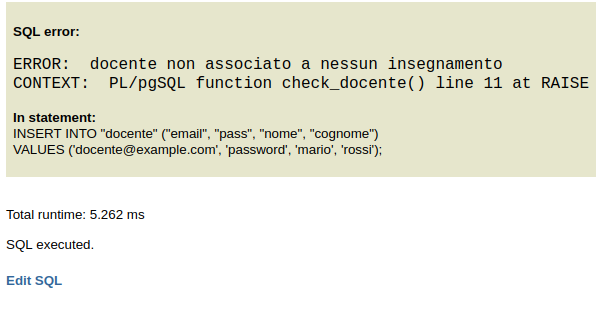
\includegraphics[width=0.9\linewidth]{images/createDocente.png}
    \label{error:createDoncenteInsert}
\end{figure}
come possiamo vedere in figura \ref{error:createDoncenteInsert} l'inserimento  non è andato a buon fine in quanto il trigger è scattato e ha impedito l'inserimento.


Se invece lanciassimo  la seguente linea dove creiamo un docente e gli associamo un insegnamento il cui id è 1 (dando pe assunto che l'insegnamento sia già presente nella tabella \textit{insegnamento}

\begin{lstlisting}[style=sqlStyle]
select * from create_docente('docen00te@example.com', 'password', 'mario', 
'rossi','2010-05-01',1);
\end{lstlisting}
otteremo il seguente risultato 
\begin{figure}[ht]
    \centering
    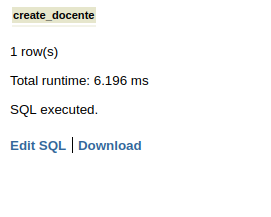
\includegraphics[width=0.2\linewidth]{images/succcesCrateDocente.png}
    \label{succ:creaDocenmtefc}
\end{figure}
notiamo come in questo caso tutto proceda correttamente e che il docente venga creato correttamente l'insegnamento riceva il proprio responabile,prima null, associato.

E se cercassimo di associare un docente ad un insegnamento con già un responsabile? 
\begin{figure}[ht]
    \centering
    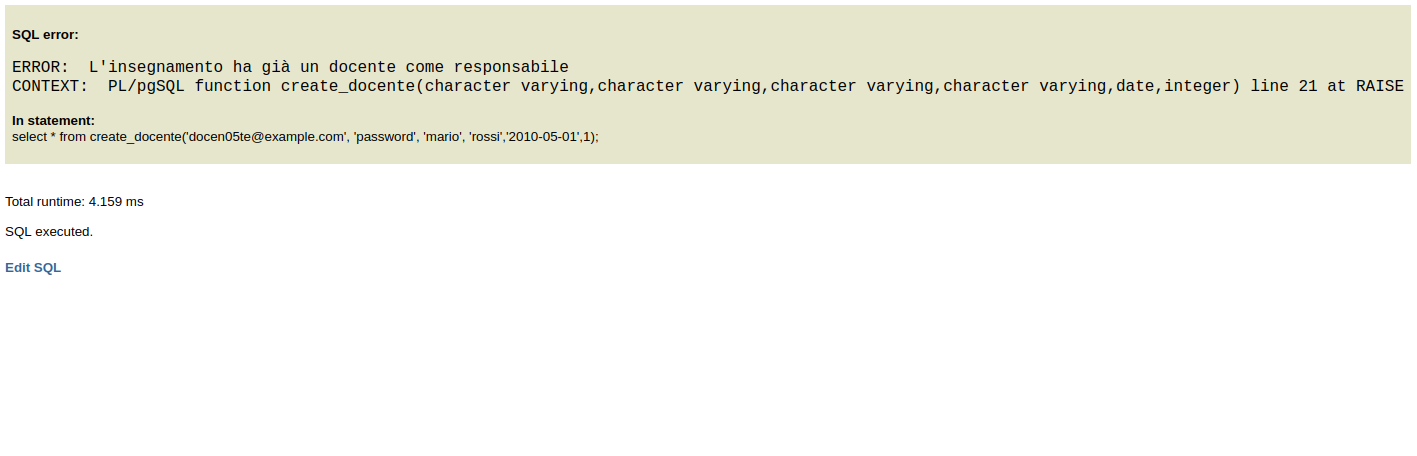
\includegraphics[width=0.9\linewidth]{images/createDocenteResponsabileError.png}
    \label{succ:creaDocenmteErrorResp}
\end{figure}

Restando in tema della colonna responsabile è doveroso notare come se si decidesse di associare più di 3 insegnamenti ad un docente  il trigger \textit{docente\_insegnamento\_tr} riportado l'errore  \textit{'Limite massimo raggiunto'}
\subsection{Carriera}
il funzionamemto delle funzioni carriera sono identiche tra loro, cambia soltanto con che criterio sono presi i voti,per questo motivo ne mostreremo soltanto uno:
\begin{lstlisting}[style=sqlStyle]
 SELECT * FROM get_carriera_valida('123456');
\end{lstlisting}
\begin{figure}[ht]
    \centering
    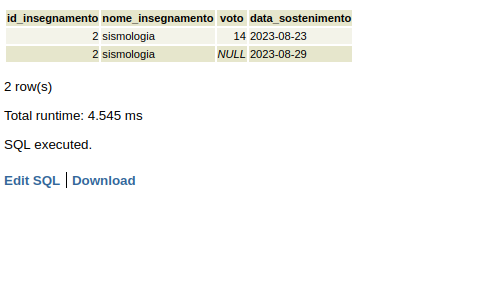
\includegraphics[width=0.9\linewidth]{images/getCarriera.png}
    \label{succ:creaDocenmteErrorResp}
\end{figure}

\subsection{Appello}
Per la creazione di un appelle ogni volta che viene eseguito controlla che non sia in conflitto con il trigger
\begin{lstlisting}[style=sqlStyle]
INSERT INTO appello VALUES ('2023-04-30','aula 200'1);
INSERT INTO appello VALUES ('2023-04-30','aula 202,2);
\end{lstlisting}
queste linee presuppongono chiaramente la presenza di due insegnamenti appartenenti allo stesso corso di laurea e con lo stesso anno consigliato 
\begin{figure}[ht]
    \centering
    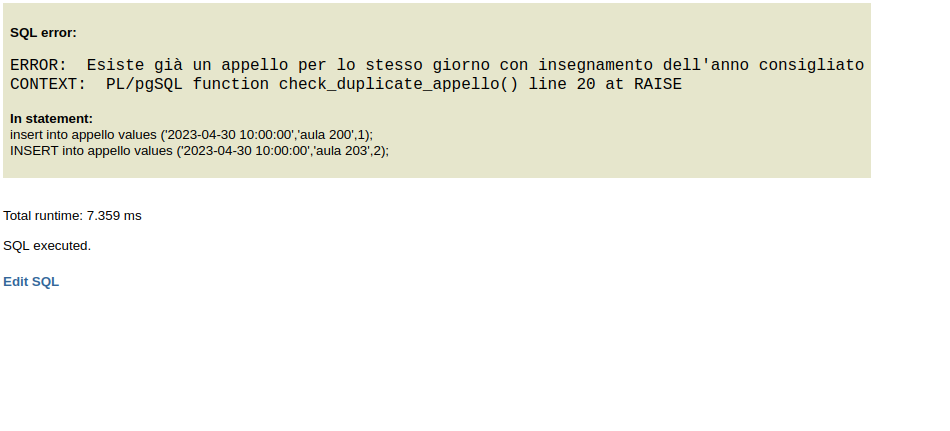
\includegraphics[width=0.9\linewidth]{images/sovrapposizione.png}
    \label{err:sovrapposizioneAppello}
\end{figure}
\subsection{CFU}
per la gestione dei voti e dei cfu utilizziamo la funzione \textit{add\_voto} la quale peremette,se uno studente è iscritto ad un esame, di assegnare un voto nella tabella appello la quale poi prosegue aggiornando i cfu in caso di voto superiore al 18.

Ipotiziamo di avere un insegnamento con id=1 e un numero di cfu pari a 6 e di avere un appello a cui lo studente è iscritto per il 2023-08-17 10:00:00. 

Questo saranno gli studenti, ci concentreremo su quello con matricola="mam":
\begin{figure}[ht]
    \centering
    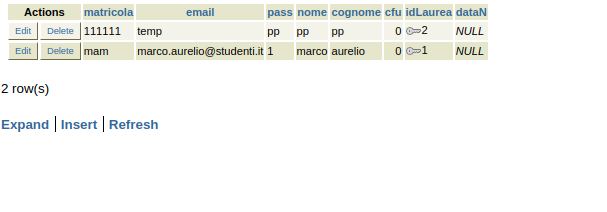
\includegraphics[width=0.9\linewidth]{images/studenti1.png}
\end{figure}
lanciando quindi la seguente  linea:
\begin{lstlisting}[style=sqlStyle]
SELECT add_voto(30, 'mam', 1, '2023-08-17 10:00:00');
\end{lstlisting}
questa linea assegnarà il voto 30 all'appello e il risulterà nella modifica dei cfu
\begin{figure}[ht]
    \centering
    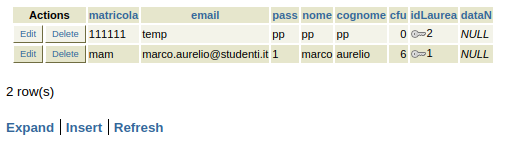
\includegraphics[width=0.9\linewidth]{images/studenti2.png}
\end{figure}
\end{document}